% !Mode:: "TeX:UTF-8"
\chapter{绪论}

\section{研究背景及意义}
    随着科技的进步,人类对自然,以及对生命有了更为深刻的认识。从显微镜的发明到DNA双链结构的提出,再到如今的21世纪,伴随着科学研究的深入,人们越来越多地发现,许多重大疾病跟基因相关,如某些癌症、一些先天性的心脏病和肥胖症。Maron等研究发现,大多数肥厚型心肌病、扩张型心肌病的病人中可发现致病基因。对于基因的研究成为了解决或预防这些疾病的关键。在人类的历史上不时出现的大规模传染病,带走了上百万人的生命,对人类的经济甚至文明都产生了巨大的影响。无论是2003年的SARS,还是2019年底的新型冠状病毒,基因都是研究这些病毒的突破点,解析了其基因的组成和作用,将极大地帮助研究人员研制出对应的抗体。每次病毒的大规模扩散,对所在国家的经济和发展都会带来巨大的损失,因此,基因研究是一项任重而道远的,属于全人类的任务。

    随着生物实验技术的进步,基因测序变得越来越方便和便宜。在美国,已经有公司推出了价格亲民的基因测序产品,人们只需花费数百美元然后在一周之内就可以知道自己的基因序列和表达情况,从而可以提前知道自己有哪些易感基因以及将来容易得哪些疾病,并以此为根据做好预防。在细胞的生物过程中,基因通过转录成信使核糖核酸(mRNA),在不同酶和氨基酸的参与下合成各种各样的蛋白质,这一过程称之为基因的表达。尽管同一生命体中的各个体细胞的基因序列是相同的,但不同的细胞仅会在特定的条件下表达特定的极少数基因。mRNA的含量越高,则其代表的基因表达水平越高。所以,研究基因的表达调控是基因组表达分析的重要内容,也有很大的意义,比如,它有助于确认病毒感染和致癌基因,并有助于确认在细胞的各个生命周期内活性基因等。通过高通量基因表达测量技术如微阵列技术(Microarray),可以测得不同mRNA的在细胞中的含量。该数据代表着基因的表达水平,因此被称为基因表达数据。通常情况下,基因表达数据的每一行代表一个基因,每一列代表一个条件或样本。

    在生物信息学中,对基因表达数据的挖掘是研究热点。基因表达数据中含有大量有用的信息。例如,在何种条件下,哪些基因是表达相似的或者存在差异?这些基因都共同参与到了哪些功能或者通路?这些基因受到了哪些调节?如何将隐藏在基因表达数据中的价值挖掘出来并利用,需要大量的计算和研究。数据挖掘领域已经大量成熟的理论和方法供人借鉴,如有监督学习的分类和无监督学习中的聚类。分类技术使得人们更方便地对新产生的数据进行分类,并在医学检测中广泛使用。通过对基因表达数据的聚类分析,可以得到研究人员感兴趣的差异基因。这些基因在不同的实验条件(如样本,时间)下,存在某种一致的表达模式。通过对这些基因的富集或旁路分析,找到这些基因的功能以及相互的调控关系。比如,Eisen 等为了推断基因的新功能,对人类的8600个基因进行了聚类,然后在聚类的结果上利用基因表达谱的相关性进行推断。Tavazoie 等使用k均值聚类算法发现了酵母转录调控网络。Tamayo 等利用相似的技术,通过对基因聚类,推断出了新基因的功能和调控网络。 

    然而,基因表达数据有两个主要特点。一,一般而言,基因的数量在几千到几万,而样本或条件的数量只有几十到几百。二,正如前面所诉,基因的表达是条件相关的。基因有可能会在多个条件下表达,也有可能在所有的条件下都没有表达。这些特点使得传统的聚类方法无法胜任,于是就引入了双聚类(Bicluster)的概念,如图\ref{fig:tradiAndBi}所示。不同于传统聚类的全局模式(Global Pattern),双聚类专注于寻找局部模式(Local Pattern),它不要求同一类基因只有在所有实验条件下才具有相似表达,而只要求在部分实验条件下具有相似的表达。找到的基因子集和条件子集就构成了一个双聚类。

    \begin{figure}[htbp]
    \setlength{\subfigcapskip}{-1bp}
    \centering
    \begin{minipage}{.9\textwidth}
    \centering
    \subfigure{}\addtocounter{subfigure}{-2}
    \subfigure{\subfigure[基因方向的传统聚类]{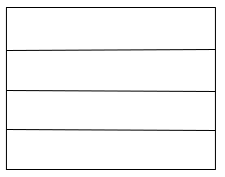
\includegraphics[width=0.29\textwidth]{1}}}
    \hspace{.1em}
    \subfigure{}\addtocounter{subfigure}{-2}
    \subfigure{\subfigure[条件方向的传统聚类]{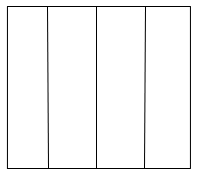
\includegraphics[width=0.25\textwidth]{2}}}
    \hspace{.1em}
    \subfigure{}\addtocounter{subfigure}{-2}
    \subfigure{\subfigure[双聚类]{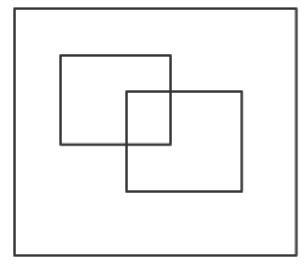
\includegraphics[width=0.25\textwidth]{3}}}
    \end{minipage}
    \vspace{0.2em}
    \caption{传统聚类与双聚类的区别}
    \label{fig:tradiAndBi}
    \end{figure}
    对于传统的聚类方法,其可以从基因或条件方向分别聚类,但是任一条件或基因都将被分配到某一类中去,这与现实中的情况是不符合的。而双聚类允许某些条件或基因不在任一类中出现。

\section{相关研究进展}
    双聚类(Bicluster)这一单词最早由Hartigan于1972年提出,但Hartigan只是在行和列两个方向上分别聚类,没有全面地阐述双聚类的概念。直到2000年,Cheng和Church将双聚类引入到基因表达数据挖掘中,提出了CC算法,并得到了较好的效果。他们提出了MSR(Mean Square Residue,均方残差)用于评价双聚类相似性。MSR越小,则表明行相似性和列相似性越高。该算法先通过不断地删除基因节点和条件节点,找到小于事先给定的MSR阈值$\delta$的双聚类,然后将其作为初始双聚类,在保证MSR不会增大的前提下,不断向其中添加基因节点和条件节点,最终得到一个双聚类结果。如果想要多个结果,算法会把之前找到的双聚类使用随机数覆盖,再重复上述操作,直到获得想要数量的双聚类。随机数的引入,会导致结果不准确,而且无法找到重叠的双聚类。2002年,Yang等对CC算法进行改进,提出了FLOC算法。算法从多个初始双聚类出发,根据最大增益的原则,来执行基因和条件节点的删除或增加。但并没有解决贪心策略带来的陷入局部最优解的问题。

    2002年,Ihmels等人提出了ISA算法(Iterative Signature Algorithm,迭代签名算法)。ISA并没有使用MSR,而是将双聚类视为转录模块,然后通过对其进行打分,迭代地修改基因集和条件集,直到无法再继续修改。同年,Tanny等提出了SAMBA(Statistical Algorithm Method For Bicluster Analysis)算法。该算法使用了图论和统计学的知识,将基因表达数据看作一个二分图,一边为基因,一边为条件。通过寻找最大稠密子图的方式来找到基因表达数据中的最大子矩阵,即双聚类。Lazzeroni 等把基因表达数据看作为背景模型与多个双聚类的叠加,并以此为基础提出了Plaid模型。

    随着大数据,集成学习,深度学习等技术的发展和普及,许多新型的双聚类分析算法涌现出来。基于 Bayesian 理论和双聚类的 Plaid 模型, Zhang 等提出了 Bayesian Plaid模型。Liu 等提出了基于GPU的统一计算设备体系结构(CUDA)的并行 GBC 算法。另外,集成学习因其在聚类方向的广泛应用,也被引入到双聚类分析中。Hanczar 等应用bagging技术提高CC和Plaid算法的结果质量。基于谱技术,Huang 等提出了SCCE(Spectral Co-Clustering Ensemble)双聚类算法。近年来的研究使得神经网络这种深度学习技术取得了突飞猛进的发展,其强大的能力不断地让人们感到惊叹。Sun 等基于深度学习技术提出了自动解码机(AutoDecoder)算法用来寻找双聚类。

    由于双聚类问题是NP难问题,通过贪婪或枚举的方法很难高效地得出结果,人们开始使用元启发式算法,如群智能算法来寻找双聚类。2004年,stanfan等人设计了一个基因表达数据双聚类分析的进化算法框架。Ken-neth Bryan等人于2006年提出了基于模拟退火算法的双聚类算法,并通过实验证明所提方法获得了质量较优的双聚类。2006年Mitra提出了多目标进化双聚类的框架,应用经典的非支配排序遗传算法( Non-dominated Sorting Genetic Algorithm-II,NSGA-II)算法,整合局部搜索策略,并提出新的定量度量方法估计双聚类的质量。2007年,Goiraldez应用最大标准区域(Maximal Standard Area,MSA)作为度量双聚类的标准,并和MSR一起应用到多目标进化算法MOEA中,提出多目标连续变化双聚类算法 (Sequential Multi objective Biclustering,SMOB),有效解决了成比例模式的双聚类问题。2013 年Carlos A. Brizula 提出了一种改进的多目标遗传双聚类算法(Enhanced Multi-objective Genetic Biclustering ,EMOGB),与其它多目标双聚类算法不同的是,他采用了一种基因和实验条件组来代表一个双聚类的编码方式, 并且在搜索双聚类的过程中减少了局部搜索环节,从而算法的执行效率有了很大的提高。
    

\section{论文主要工作}
    因为基因表达数据上双聚类分析的困难性和重要性,过去提出的大量算法都有各自的侧重点。有关基于元启发式的双聚类分析算法,缺少一个较为完整的完整的分析工作。本文以提高双聚类结果的质量指标和生物意义为目标,结合混合元启发式方法和多目标优化方法,对双聚类分析这一问题进行了综合比较研究。本文主要工作如下:
    \begin{itemize}
       \item[(1)] {考虑到布谷鸟搜索算法和萤火虫算法的优势互补,本文提出了一种基于布谷鸟搜索和萤火虫算法的混合双聚类分析算法(Cuckoo Search and Firfly Algorithm hybrid Biclustering,CSFAB)。首先,将均方残差,基因容量和样本容量的权重之和作为适应值函数。然后将连续的解转换成比特串来表示双聚类,经过几种混合方式的比较之后,选择了最佳的混合方案。最后在四个常用且数据规模大小不一的基因表达数据集上,通过实验对算法的有效性进行了分析和验证。}

       \item[(2)] {双聚类分析其实是多目标优化问题。本文提出了一种多目标细菌觅食算法的双聚类分析算法(Multi-object Bacterial Foraging Algorithm Biclustering,MOBFOB)。算法将均方残差,基因容量和样本容量看作待优化指标,并按照被支配次数对种群排序。以细菌觅食算法为指导,不断地寻找占优的双聚类,并将其保存在外部集合中。最后在四个基因表达数据集上,通过实验对算法的有效性进行了验证。}
       
    \end{itemize}

\section{论文组织结构}
    本文首先对基因表达数据和双聚类分析等相关基础知识进行阐述。然后从单目标优化,混合优化和多目标优化等方面,研究了以群智能算法如布谷鸟搜索算法、萤火虫算法和细菌觅食算法为框架的双聚类算法。最后对本文的工作进行了总结和展望。全文共有五章,本文各章节内容安排如下:

    第一章从生物背景知识出发,讨论了基因研究的重要性以及双聚类的作用和发展现状。双聚类克服了常规聚类与基因表达数据之间的矛盾,能更好的挖掘出有价值的基因子集和条件子集。群智能算法由于其快速且效果更好,在双聚类分析中得到了很广泛地应用。

    第二章先是更具体地讨论的基因表达数据的数学形式,以及双聚类的定义、类型和结构。接着将双聚类算法分为了基于质量评价指标和基于模型两种。然后,对于双聚类结果,讨论了其质量验证指标和生物验证指标。最后分别介绍了本文所关注的群智能算法。

    第三章为了解决普通双聚类算法的质量评价指标不足和生物意义不明显的缺点,本文将布谷鸟算法与萤火虫算法进行了融合,并提出了CSFAB双聚类算法。通过实验,确定了融合的最佳方案,并从质量评价指标和生物评价指标的角度进行了比较分析。

    第四章首先介绍了多目标优化的基本概念,接着将细菌觅食算法按照多目标优化和双聚类的特点进行了改进,包括适应值函数,以及互不支配时的比较规则,并提出了MOBFOB算法。最后根据适应值曲线和生物指标对算法进行了分析。
    
    第五章对全文工作进行了总结和展望。
